%!TEX root = ./BPM17.tex

\section{Evaluation} % (fold)
\label{sec:evaluation}
%%%% CONTENT

In this section, we provide an evaluation of our predictive business process monitoring techniques based on a-priori knowledge. In particular, we check: (i) whether the \nocycle algorithm leveraging knowledge about the structure of the process execution traces (and in particular about the presence of cycles) actually improves the predictions; and (ii) whether the \protrack algorithm is able to leverage a-priori knowledge to improve the performance of the LSTM model.

\subsection{Event Logs}
\label{ssec:datasets}
%presentation of <datasets, constraints>

\begin{table}[t]
	\centering
	 \begin{scriptsize}
	\begin{tabular}{l|c|c|c|c|c}
		\toprule
			   %  & 		         		     & 		               & %\multicolumn{3}{c}{\textbf{Average}} \\ \cmidrule{5-7}
		\textbf{Log} &\textbf{\#Tr.}  & \textbf{\#Act.}  & \textbf{avg-TL} & \textbf{avg-CR}  & \textbf{Spars.}\\
		\midrule
		EnvLog      & 937    & 299   & 41      & 0.14 & 0.3191 \\
		HelpDesk    & 3804   & 9     & 3.6       & 0.22 & 0.0024 \\
		BPIC11       & 1\,143    & 355   & 54       & 5.05 & 0.3897 \\
		BPIC12       & 13\,087   & 7     & 7.5     & 1.35 & 0.0007 \\
		BPIC13       & 7\,554   & 13    & 7       & 1.45 & 0.0017 \\
		BPIC17       & 31\,509  & 27    & 18     & 0.46 & 0.0009 \\
		\bottomrule
	\end{tabular}
	\end{scriptsize}
	\caption{The event logs}
	\label{table:dataset}
\end{table}

For the evaluation of the techniques, we used six real-life event logs. Four of them were provided for the BPI Challenges (BPIC) 2011~\cite{bpichallenge2011}, 2012~\cite{bpichallenge2012}, 2013~\cite{bpichallenge2013}, and 2017~\cite{bpichallenge2017}, respectively. We also used two additional event logs, one pertaining to an environmental permit application process (``WABO''), used in the context of the CoSeLoG project~\cite{EnvironmentalLog} (\emph{EnvLog} for short in this paper), and another containing cases from a ticketing management process of the help desk of an Italian software company (\emph{Helpdesk}\footnote{\url{https://data.mendeley.com/datasets/39bp3vv62t/1}} for short).

\begin{enumerate}
	\item \textbf{Environment permit log} (\emph{EnvLog}) is the log containing data that come from Dutch municipality\footnote{\url{https://data.4tu.nl/repository/uuid:e8c3a53d-5301-4afb-9bcd-38e74171ca32}}. The cases are the application process of the environment permits. It contains 937 cases, 38.944 events, and 381 events types.
	\item \textbf{Helpdesk} is the dataset containing events from a ticketing management process of the help desk of an Italian software company. The process consists of 9 activities, and all cases start with the insertion of a new ticket into the ticketing
	management system. Each case ends when the issue is resolved and the ticket is closed. This log contains 3804 process instances (a.k.a "cases") and 13710 events
	\item \textbf{BPI 11 log} is the famous in process mining log taken from Dutch Academic Hospital. The cases of the log correspond to the Gynaecology department of the hospital. Phases consist of the diagnosis and treatment of the patient. Some attributes are repeating as the procedures could take place few number of times. As the log contains sensitive information it was anonymized.
	\item \textbf{BPI 12 subprocess W dataset\footnote{\url{http://data.4tu.nl/repository/uuid:3926db30-f712-4394-aebc-75976070e91f}.}} This is the part of the BPI 2012 challenge, that contains a real-life log, taken from a Dutch Financial Institute. The process represented in the event log is an application process for a personal loan or overdraft within a global financing organization. 
	
	This log is contains a lot of information the usual prediction task system would bot be interested in. The paper\cite{niek96732} proposed to cut the log down to the traces what contain events that are manualy executed. So the pre-processed log was taken from their github repository\footnote{\url{https://github.com/verenich/ProcessSequencePrediction/tree/master/data}}.
	
	\item \textbf{BPI 13 log\footnote{\url{http://www.win.tue.nl/bpi/doku.php?id=2013:challenge}}} was prepared by Volvo IT in Belgium. Log consist of incident and problem management from their system "VINST".   
	
	\item \textbf{BPI 17 log\footnote{\url{http://data.4tu.nl/repository/uuid:5f3067df-f10b-45da-b98b-86ae4c7a310b}}} is a process taken from Dutch financial institute. In particular the process we used it a loan applications. It has much more data that other logs that we considered. 
		
	
\end{enumerate}

The characteristics of these logs are summarized in Table~\ref{table:dataset}. For each log, we report the total number of traces, the number of activity labels (i.e., the size of the activity set of the log), the average trace length (avg-TL), the average number of repetitions of all cycles in the log (avg-CR), and the ratio between the number of activity labels and the number of traces, indicating the sparsity of the activity labels over the log.
%Concerning the test set we did use 67\% of the whole dataset for training. Then we selected for testing a relevant subset of the remaining 33\%  satisfying, for each dataset, the additional (a-priori) knowledge, described in terms of LTL formulas. To maximize the size of the testing set we selected LTL formulas satisfied by a conspicuous number of traces among the remaining 33\% ones.

%For the a-priori knowledge, we divided the event logs in training and testing set and we selected LTL formulas satisfied by a conspicuous number of traces in the testing set. For each event log we selected a conjunction of \textit{strong} and of \textit{weak} formulas, which respectively strongly and weakly constrain the trace. For instance a formula LTL of the type $\sometime A$ is weaker than a formula $\always(A \imp \sometime B) \wedge \sometime A$ since the latter imposes the occurrence of both $A$ and $B$ and of a temporal relationships between them. The schematic form of the formulas used in the evaluation is reported in Table~\ref{table:apriori}, where - for the sake of readability - we replace the original activity names with propositional atoms.
% reported in Table~\ref{table:apriori} by means of LTL (linear time temporal logic) formulas.


%experiment setup table




\subsection{Experimental Procedure}
\label{ssec:procedure}
%presentation of baseline + metrics



In order to evaluate the techniques presented in the paper, we adopted the following procedure. For each event log:
\begin{enumerate}
%	\item We divided all our event logs in three parts: a \textbf{training set} composed of the 67\% of the whole event log and two \textbf{testing sets}, a so-called strong-apriori testing set and a so-called weak-apriori testing set, respectively composed of the subsets of the remaining 33\% which satisfy the strong and weak a-priori knowledge reported in Table~\ref{table:apriori}\footnote{Note that strong-apriori and weak-apriori are not necessarily disjoint.}.
\item We divided the event log in two parts: a \textbf{training set} composed of the 67\% of the whole event log and a \textbf{testing set}, composed of the remaining 33\%.
\item We derived the a-priori knowledge on the traces of the testing set as follows. We randomly selected 10\% of traces of the testing set. From each trace, we extracted 4 prefixes of lengths corresponding to the 4 integers in the interval $\left[mid-2,mid+2\right]$, where $mid$ is half of the median of the trace lengths. We derived all suffixes of these prefixes and we used the DeclareMiner ProM plug-in~\cite{Maggi2012} to discover LTL rules satisfied in all those suffixes. Then, we defined 2 conjunctive rules describing a \textit{strong a-priori knowledge} and a \textit{weak a-priori knowledge}, which respectively strongly and weakly constrain the traces. In particular, we discovered rules of type $\sometime A$ (which imposes the occurrence of $A$) for defining the weak a-priori knowledge and rules of type $\always(A \imp \sometime B) \wedge \sometime A$ (which imposes the occurrence of both $A$ and $B$ and that every occurrence of $A$ is followed by an occurrence of $B$) for defining the strong a-priori knowledge. For the weak a-priori knowledge, we randomly selected from the discovered rules one, two or three (depending on the average length of the traces in the log) rules of type $\sometime A$ and we composed them into a single conjunctive formula. Similarly, for the strong a-priori knowledge, we randomly selected one, two or three rules from the discovered rules of type $\always(A \imp \sometime B) \wedge \sometime A$ and we composed them into a single conjunctive formula. We followed this systematic procedure for defining the a-priori knowledge, to limit the bias of the selected rules while guaranteeing that they are satisfied in a reasonable number of traces of the testing set. The schematic form of the rules used in the evaluation is reported in Table~\ref{table:apriori}, where - for the sake of readability - we replace the original activity names with single characters. Starting from strong and weak a-priori knowledge, we built a \emph{strong a-priori testing set} and a \emph{weak a-priori testing set}, respectively composed of the subsets of traces of the testing set that satisfy strong and weak a-priori knowledge.
\item  we compared \nocycle and \protrack \footnote{We set $bSize$ to $3$ and, for the coefficient in charge of weakening the probabilities of activities in a cycle, we used the exponential formula ($e^{j}$, where $j$ is the number of cycle repetitions).} against a baseline provided by the technique presented in \cite{niek96732}. For each technique, we computed: (i) the length of the predicted suffixes; and (ii) their similarity with the prediction ground truth measured using the Damerau-Levenshtein similarity~\cite{Damerau:1964:TCD:363958.363994}.
\end{enumerate}
\begin{table}[t!]
	\centering	
	\begin{scriptsize}
	\begin{tabular}{l|c|c}
		\toprule
		\textbf{Log}  & \textbf{A-priori Strong} & \textbf{A-priori Weak} \\
		\midrule
		EnvLog     & $\always(a \imp \sometime b) \wedge \sometime a \wedge \always(c \imp \sometime d) \wedge \sometime c$  & $\sometime a \wedge \sometime c$ \\
		HelpDesk   & $\always(e \imp \sometime f) \wedge \sometime e$ & $\sometime e$\\
		BPIC11      & $\always(g \imp \sometime h) \wedge \sometime g \wedge \always(i \imp \sometime l) \wedge \sometime i \wedge \always(m \imp \sometime n) \wedge \sometime m$ &
		$\sometime i \wedge \sometime h \wedge \sometime o$		\\
		BPIC12      & $\always(p \imp \sometime q) \wedge \sometime p$ & $\sometime p$   \\
		BPIC13      & $\always(r \imp \sometime s) \wedge \sometime r \wedge \always(t \imp \sometime r) \wedge \sometime t$ & $\sometime s \wedge \sometime r$ \\
		BPIC17      & $\always(u \imp \sometime v) \wedge \sometime u$  & $\sometime u$  \\
		\bottomrule
	\end{tabular}
	\end{scriptsize}
	\caption{The a-priori knowledge.}
	\label{table:apriori}
\end{table}
The experiments have been performed both on a GPU Tesla K40c and on a conventional laptop CPU on Code i5. As for the LSTM training settings we used the ones identified by Tax et al.~\cite{niek96732} as the most performing ones for facing the problem of predicting sequences of future activities.\footnote{We used an architecture characterized by two LSTM layers. The algorithm used is the Adam learning algorithm with categorical cross entropy loss and the dropout coefficient has been set to 0.2.} The time required for training the LSTM neural network is about 2 minutes per epoch using the GPU and 15 minutes using the CPU. The inference time for \nocycle %(not modified version of LSTM model prediction)
 is about 0.1-2 seconds per trace (depending on the log), whereas the inference time for \protrack is 4 times higher on average.


%We used two hidden layers for the network: one shared layer for sequence of activities and time feature, and two joint layers for activities and time sequence preceding output layer. The dropout coefficient is 0.2, and the network is equipped Adam learning algorithm. These parameters shown to work best for the problem at hand\cite{niek96732}. We also have 500 maximum number of epoch, and categorical cross entropy loss.

\subsection{Results and Discussion}
\label{ssec:results}
%big table of results + comment the table (comment on logs with cycles, comment that and on why protrack traces are longer than backtrack, ... )

Tables~\ref{table:results-strong} and~\ref{table:results-weak} report, for each event log, the performances of the two techniques we propose on the strong a-priori and weak a-priori testing sets. Also, the same results are displayed on the graph~\ref{figure:results}. The results for both testing sets are compared with the baseline presented in~\cite{niek96732}. For each log, we provide the average Damerau-Levenshtein similarity between the predicted sequence (in square brackets, its average length) and the ground truth (column 5). The best average Damerau-Levenshtein similarity for each log is emphasized in gray. Column 6 reports the number of traces tested while column 7 specifies the range of the prefix lengths used for the specific event log. %The prefixes range is chosen around middle point of the average lengths of the traces.

\newcommand{\maxf}[1]{{\cellcolor[gray]{0.8}} #1}

%\begin{table}[h]
%	\centering
%	\sisetup{detect-weight=true,detect-inline-weight=math}
%	\begin{tabular}{lS[table-unit-alignment = right]s[table-unit-alignment = left]S[table-unit-alignment = right]s[table-unit-alignment = left]S[table-unit-alignment = right]s[table-unit-alignment = left]S[table-unit-alignment = right]s[table-unit-alignment = left]Sc}
%		\toprule
%		\textbf{Log}  & \multicolumn{2}{c}{\textbf{Baseline}} & \multicolumn{2}{c}{\nocycle} & \multicolumn{2}{c}{\backtrack}  & \multicolumn{2}{c}{\protrack} & \textbf{Groundtruth}  & \textbf{Prefix} \\\hline
%		EnvLog        & \maxf{0.22}&[\num{25.99}]   & 0.22&[\num{25.49}]        & 0.22&[\num{26.26}]                            & 0.22&[\num{27.67}]          & 33.61                 & 2-20         \\
%		HelpDesk      & 0.65&[\num{1.26}]           & 0.65&[\num{1.26}]         & \maxf{0.77}&[\num{1.15}]                      & \maxf{0.77}&[\num{1.15}]    & 1.71                  & 2-Max         \\
%		BPI11         & 0.19&[\num{199.00}]         & 0.24&[\num{42.59}]        & \maxf{0.34}&[\num{57.61}]                     & 0.25&[\num{145.86}]         & 89.41                 & 10 \\
%		BPI13         & 0.58&[\num{32.30}]          & \maxf{0.60}&[\num{2.60}]  & 0.57&[\num{1.76}]                             & 0.53&[\num{2.29}]           & 1.92                  & 3-10          \\
%		BPI12         & 0.08&[\num{58.74}]          & 0.26&[\num{2.10}]         & 0.16&[\num{1.33}]                             & \maxf{0.32}&[\num{2.75}]    & 7.22                  & 3-10           \\
%		BPI17         & 0.40&[\num{13.62}]          & 0.40&[\num{13.62}]        & \maxf{0.41}&[\num{13.46}]                     & 0.40&[\num{13.62}]          & 9.39                  & 5        \\
%		\bottomrule
%	\end{tabular}
%	\caption{Results related to predictions.}
%		\label{table:results}
%\end{table}

\begin{table}[t]
	\centering
	\sisetup{detect-weight=true,detect-inline-weight=math}
\begin{scriptsize}
	\begin{tabular}{lS[table-unit-alignment = right]s[table-unit-alignment = left]S[table-unit-alignment = right]s[table-unit-alignment = left]S[table-unit-alignment = right]s[table-unit-alignment = left]S[table-unit-alignment = right]s[table-unit-alignment = right]s[table-unit-alignment = left]Sc}
		\toprule
		\textbf{Log}  & \multicolumn{2}{c}{\textbf{Baseline}} & \multicolumn{2}{c}{\nocycle}  & \multicolumn{2}{c}{\protrack} & \textbf{Groundtruth} & \textbf{Tested} & \textbf{Prefix} \\\hline
		EnvLog        & \maxf{0.250}&[\num{17.4}]   & \maxf{0.250}&[\num{17.4}]                      & 0.070&[\num{95.00}]          & 29.40              & 80   & 19-22         \\
		HelpDesk      & 0.551&[\num{1.44}]           & 0.551&[\num{1.44}]                       & \maxf{0.831}&[\num{2.36}]    & 3.00         & 576         & 2-5          \\
		BPIC11         & 0.204&[\num{199.00}]         & \maxf{0.281}&[\num{199.00}]                      & 0.274&[\num{198.00}]         & 117.11          & 144       & 13-16 \\
		BPIC12         & 0.071&[\num{47.07}]          & 0.387&[\num{6.86}]                       & \maxf{0.416}&[\num{7.53}]    & 10.95          & 1\,548        & 2-5            \\
		BPIC13         & 0.116&[\num{100.80}]          & 0.502&[\num{14.71}]                & \maxf{0.596}&[\num{6.13}]           & 7.15       & 3\,209           & 2-5          \\
		BPIC17         & 0.448&[\num{11.78}]          & 0.448&[\num{11.78}]                      & \maxf{0.510}&[\num{15.14}]          & 16.01        & 10\,153          & 6-9        \\
		\bottomrule
	\end{tabular}
\end{scriptsize}
	\caption{Prediction results on the strong a-priori testing set}
	\label{table:results-strong}
\end{table}


\begin{table}[t]
	\centering
	\sisetup{detect-weight=true,detect-inline-weight=math}
\begin{scriptsize}
	\begin{tabular}{lS[table-unit-alignment = right]s[table-unit-alignment = left]S[table-unit-alignment = right]s[table-unit-alignment = left]S[table-unit-alignment = right]s[table-unit-alignment = left]S[table-unit-alignment = right]s[table-unit-alignment = right]s[table-unit-alignment = left]Sc}
		\toprule
		\textbf{Log}  & \multicolumn{2}{c}{\textbf{Baseline}} & \multicolumn{2}{c}{\nocycle}  & \multicolumn{2}{c}{\protrack} & \textbf{Groundtruth}  & \textbf{Tested} & \textbf{Prefix} \\\hline
		EnvLog        & \maxf{0.246}&[\num{18.22}]   & \maxf{0.246}&[\num{18.22}]                      & 0.084&[\num{89.91}]          & 31.31              & 108  & 19-22         \\
		HelpDesk      & 0.551&[\num{1.44}]           & 0.551&[\num{1.44}]                       & \maxf{0.747}&[\num{2.14}]    & 3.00             & 576    & 2-5         \\
		BPIC11         & 0.220&[\num{199.00}]         & \maxf{0.292}&[\num{199.00}]                      & 0.282&[\num{197.4}]         & 112.66            & 450     & 13-16 \\
		BPIC12         & 0.100&[\num{48.08}]          & 0.263&[\num{6.81}]                       & \maxf{0.264}&[\num{7.00}]    & 8.33       &      3\,179     & 2-5           \\
		BPIC13         & 0.130&[\num{95.19}]          & 0.459&[\num{14.92}]                & \maxf{0.569}&[\num{5.14}]           & 5.85         &  4\,364         & 2-5          \\
		BPIC17         & 0.448&[\num{11.78}]          & 0.448&[\num{11.78}]                      & \maxf{0.469}&[\num{14.00}]          & 16.01        & 10\,153          & 6-9        \\
		\bottomrule
	\end{tabular}
\end{scriptsize}
	\caption{Prediction results on the weak a-priori testing set}
	\label{table:results-weak}
\end{table}



\begin{figure}[!ht]
	\begin{center}  
		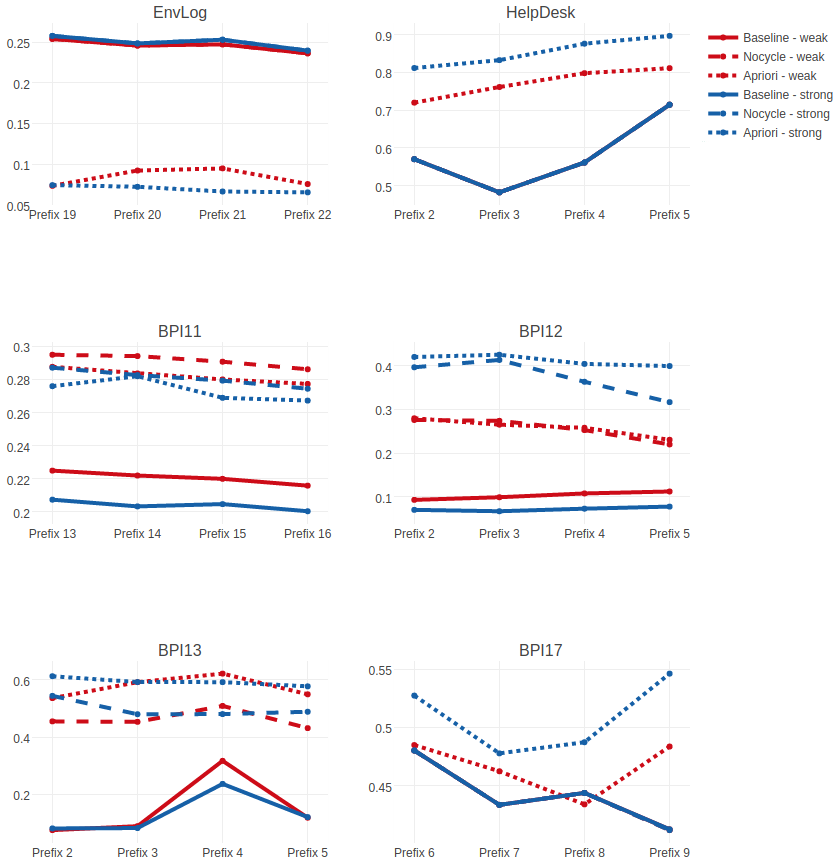
\includegraphics[width=\textwidth]{2_evaluation.png}
		\caption{Graphical representation of evaluation}
		\label{figure:results}
	\end{center}
\end{figure}


The tables show that the proposed algorithms outperform the baseline in most of the logs.
The presence of cycles in the logs has a strong impact on the performance of the \nocycle algorithm. In particular, if the logs have an average number of cycle repetitions smaller than $0.5$, as in the case of EnvLog, HelpDesk and BPIC17, then \nocycle does not show any improvement over the baseline. Therefore, we can conclude that \nocycle correctly deals with the presence of cycles in the logs to improve the predictions.




%Concerning the ability of \protrack to leverage the regularity of the logs, it is evident that the best improvements obtained by the \protrack algorithm refer to event logs that have a small activity set (small number of activity labels) and not HelpDesk and BPIC13 in our experiments.

\protrack perform worse on logs EnvLog and the BPIC11. The reason for this can be explained by the fact that, in these two logs, activity labels are sparse with an unusually high number of labels with respect to the number of traces. Indeed, Table~\ref{table:dataset} shows that the ratio between the number of activity labels and the number of traces (column 8) for these logs is higher with respect to the other logs.
%While a full investigation of the impact of the log characteristics over the performance of LSTM-based techniques is out of the scope for this paper and is left to future work, we can already say that logs characterized by a high degree of sparsity of activity labels (and, therefore, containing sparse behaviors) are unlikely candidates to benefit from the proposed techniques.
We can also notice that the availability of highly constraining rules in the a-priori knowledge improves the performance of \protrack. Therefore, we can conclude that \protrack is able to correctly leverage a-priori knowledge in a way that it performs better when the activity set of the log is not particularly large (and the log does not contain sparse behaviors) and when the a-priori knowledge constrains more the process behavior.




%To sum up, the evaluation shows that both the \nocycle and the \protrack techniques actually improve the performance of the baseline approach and they are particularly suitable to be used when the event logs present several cycles or when the alphabet is not extremely large, respectively.

% , we can observe
% 	\item {Big performance for apriori shown on logs which have small alphabet and not much cycles (helpdesk, bpi13)}
% 	\item {For logs mentioned above and for the same reasons, the difference between STRONG and WEAK formulas are bigger(STRONG performs very good). }
% 	\item {Applying STRONG formulas gives better results as they more constraining in most cases.}


%\todoincg{shall we add a sentence in terms of lessons learned or is this enough?}
% \subsection{Discussion}
%
% \begin{itemize}
% 	% \item{Environment permit, BPI11 do not improve with apriori knowledge because the training data is too sparse and alphabet size is too big.}
% 	% \item{If there are no cycles (in our logs it is less than 0.5 per trace) there is no improvement for NOCycle technique. (Examples env permit, helpdesk, bpi17)}
% 	\item {Big performance for apriori shown on logs which have small alphabet and not much cycles (helpdesk, bpi13)}
% 	\item {For logs mentioned above and for the same reasons, the difference between STRONG and WEAK formulas are bigger(STRONG performs very good). }
% 	\item {Applying STRONG formulas gives better results as they more constraining in most cases.}
%
% \end{itemize}

% \label{ssec:discussion}
% "lessons learned"': when we have cycles in the log, we should use the cycle approach, when the average lenght of the log is high then use protrack, ...

% section evaluation (end) 